% Template for PLoS
% Version 3.5 March 2018
%
% % % % % % % % % % % % % % % % % % % % % %
%
% -- IMPORTANT NOTE
%
% This template contains comments intended 
% to minimize problems and delays during our production 
% process. Please follow the template instructions
% whenever possible.
%
% % % % % % % % % % % % % % % % % % % % % % % 
%
% Once your paper is accepted for publication, 
% PLEASE REMOVE ALL TRACKED CHANGES in this file 
% and leave only the final text of your manuscript. 
% PLOS recommends the use of latexdiff to track changes during review, as this will help to maintain a clean tex file.
% Visit https://www.ctan.org/pkg/latexdiff?lang=en for info or contact us at latex@plos.org.
%
%
% There are no restrictions on package use within the LaTeX files except that 
% no packages listed in the template may be deleted.
%
% Please do not include colors or graphics in the text.
%
% The manuscript LaTeX source should be contained within a single file (do not use \input, \externaldocument, or similar commands).
%
% % % % % % % % % % % % % % % % % % % % % % %
%
% -- FIGURES AND TABLES
%
% Please include tables/figure captions directly after the paragraph where they are first cited in the text.
%
% DO NOT INCLUDE GRAPHICS IN YOUR MANUSCRIPT
% - Figures should be uploaded separately from your manuscript file. 
% - Figures generated using LaTeX should be extracted and removed from the PDF before submission. 
% - Figures containing multiple panels/subfigures must be combined into one image file before submission.
% For figure citations, please use "Fig" instead of "Figure".
% See http://journals.plos.org/plosone/s/figures for PLOS figure guidelines.
%
% Tables should be cell-based and may not contain:
% - spacing/line breaks within cells to alter layout or alignment
% - do not nest tabular environments (no tabular environments within tabular environments)
% - no graphics or colored text (cell background color/shading OK)
% See http://journals.plos.org/plosone/s/tables for table guidelines.
%
% For tables that exceed the width of the text column, use the adjustwidth environment as illustrated in the example table in text below.
%
% % % % % % % % % % % % % % % % % % % % % % % %
%
% -- EQUATIONS, MATH SYMBOLS, SUBSCRIPTS, AND SUPERSCRIPTS
%
% IMPORTANT
% Below are a few tips to help format your equations and other special characters according to our specifications. For more tips to help reduce the possibility of formatting errors during conversion, please see our LaTeX guidelines at http://journals.plos.org/plosone/s/latex
%
% For inline equations, please be sure to include all portions of an equation in the math environment.  For example, x$^2$ is incorrect; this should be formatted as $x^2$ (or $\mathrm{x}^2$ if the romanized font is desired).
%
% Do not include text that is not math in the math environment. For example, CO2 should be written as CO\textsubscript{2} instead of CO$_2$.
%
% Please add line breaks to long display equations when possible in order to fit size of the column. 
%
% For inline equations, please do not include punctuation (commas, etc) within the math environment unless this is part of the equation.
%
% When adding superscript or subscripts outside of brackets/braces, please group using {}.  For example, change "[U(D,E,\gamma)]^2" to "{[U(D,E,\gamma)]}^2". 
%
% Do not use \cal for caligraphic font.  Instead, use \mathcal{}
%
% % % % % % % % % % % % % % % % % % % % % % % % 
%
% Please contact latex@plos.org with any questions.
%
% % % % % % % % % % % % % % % % % % % % % % % %

\documentclass[10pt,letterpaper]{article}
%\usepackage[top=0.85in,left=2.75in,footskip=0.75in]{geometry}
\usepackage[top=0.85in,left=1.75in,footskip=0.75in]{geometry}

% amsmath and amssymb packages, useful for mathematical formulas and symbols
\usepackage{amsmath,amssymb}

% Use adjustwidth environment to exceed column width (see example table in text)
\usepackage{changepage}

% Use Unicode characters when possible
\usepackage[utf8x]{inputenc}

% textcomp package and marvosym package for additional characters
\usepackage{textcomp,marvosym}

% cite package, to clean up citations in the main text. Do not remove.
\usepackage{cite}

% Use nameref to cite supporting information files (see Supporting Information section for more info)
\usepackage{nameref,hyperref}

% line numbers
\usepackage[right]{lineno}

% ligatures disabled
\usepackage{microtype}
\DisableLigatures[f]{encoding = *, family = * }

% color can be used to apply background shading to table cells only
\usepackage[table]{xcolor}

% array package and thick rules for tables
\usepackage{array}

% create "+" rule type for thick vertical lines
\newcolumntype{+}{!{\vrule width 2pt}}

% create \thickcline for thick horizontal lines of variable length
\newlength\savedwidth
\newcommand\thickcline[1]{%
  \noalign{\global\savedwidth\arrayrulewidth\global\arrayrulewidth 2pt}%
  \cline{#1}%
  \noalign{\vskip\arrayrulewidth}%
  \noalign{\global\arrayrulewidth\savedwidth}%
}

% \thickhline command for thick horizontal lines that span the table
\newcommand\thickhline{\noalign{\global\savedwidth\arrayrulewidth\global\arrayrulewidth 2pt}%
\hline
\noalign{\global\arrayrulewidth\savedwidth}}


% Remove comment for double spacing
%\usepackage{setspace} 
%\doublespacing

% Text layout
\raggedright
\setlength{\parindent}{0.5cm}
\textwidth 5.25in 
\textheight 8.75in

% Bold the 'Figure #' in the caption and separate it from the title/caption with a period
% Captions will be left justified
\usepackage[aboveskip=1pt,labelfont=bf,labelsep=period,justification=raggedright,singlelinecheck=off]{caption}
\renewcommand{\figurename}{Fig}

% Use the PLoS provided BiBTeX style
\bibliographystyle{plos2015}

% Remove brackets from numbering in List of References
\makeatletter
\renewcommand{\@biblabel}[1]{\quad#1.}
\makeatother

%%% BOXED SECTIONS by Tessa Pierce :) (with help from the internet)
\usepackage{color}
\definecolor{lightgray}{gray}{0.90}

\newcommand\greybox[1]{%
  \vskip\baselineskip%
  \par\noindent\colorbox{lightgray}{%
    \begin{minipage}{\textwidth}#1\end{minipage}%
  }%
  \vskip\baselineskip%
}
%% codeblock settings
\usepackage{listings}
\lstset{
  basicstyle=\small,
  xleftmargin=.05\textwidth, xrightmargin=.05\textwidth
}


%%% ADDING INLINE FIGURES -- added by taylor reiter, remove before submission
\usepackage{graphicx}
\graphicspath{ {./figures/} }
%%% end add inline figures

% Header and Footer with logo
\usepackage{lastpage,fancyhdr,graphicx}
\usepackage{epstopdf}
%\pagestyle{myheadings}
\pagestyle{fancy}
\fancyhf{}
%\setlength{\headheight}{27.023pt}
%\lhead{\includegraphics[width=2.0in]{PLOS-submission.eps}}
\rfoot{\thepage/\pageref{LastPage}}
\renewcommand{\headrulewidth}{0pt}
\renewcommand{\footrule}{\hrule height 2pt \vspace{2mm}}
\fancyheadoffset[L]{2.25in}
\fancyfootoffset[L]{2.25in}
\lfoot{\today}

%% Include all macros below

\newcommand{\lorem}{{\bf LOREM}}
\newcommand{\ipsum}{{\bf IPSUM}}

%% END MACROS SECTION


\begin{document}
\vspace*{0.2in}

% Title must be 250 characters or less.
\begin{flushleft}
{\Large
\textbf\newline{A road map for working with biological sequencing data} % Please use "sentence case" for title and headings (capitalize only the first word in a title (or heading), the first word in a subtitle (or subheading), and any proper nouns).
}
\newline
% Insert author names, affiliations and corresponding author email (do not include titles, positions, or degrees).


Taylor Reiter 0000-0002-7388-421X\textsuperscript{1,2},
%Name2 Surname\textsuperscript{1},
C. Titus Brown 0000-0001-6001-2677\textsuperscript{1},
N. Tessa Pierce 0000-0002-2942-5331\textsuperscript{1,*},
\\
\bigskip
\textbf{1} Department of Population Health and Reproduction, University of California, Davis, CA, USA
\\
\textbf{2} Food Science Graduate Group, University of California, Davis, CA, USA
\\
\bigskip

% Insert additional author notes using the symbols described below. Insert symbol callouts after author names as necessary.
% 
% Remove or comment out the author notes below if they aren't used.
%
% Primary Equal Contribution Note
%\Yinyang These authors contributed equally to this work.

% Additional Equal Contribution Note
% Also use this double-dagger symbol for special authorship notes, such as senior authorship.
%\ddag These authors also contributed equally to this work.

% Current address notes
%\textcurrency Current Address: Dept/Program/Center, Institution Name, City, State, Country % change symbol to "\textcurrency a" if more than one current address note
% \textcurrency b Insert second current address 
% \textcurrency c Insert third current address

% Deceased author note
%\dag Deceased

% Group/Consortium Author Note
%\textpilcrow Membership list can be found in the Acknowledgments section.

% Use the asterisk to denote corresponding authorship and provide email address in note below.
* ntpierce@ucdavis.edu

\end{flushleft}
% Please keep the abstract below 300 words
\section*{Abstract}
Lorem ipsum dolor sit amet, %consectetur adipiscing elit. Curabitur eget porta erat. Morbi consectetur est vel gravida pretium. Suspendisse ut dui eu ante cursus gravida non sed sem. Nullam sapien tellus, commodo id velit id, eleifend volutpat quam. Phasellus mauris velit, dapibus finibus elementum vel, pulvinar non tellus. Nunc pellentesque pretium diam, quis maximus dolor faucibus id. Nunc convallis sodales ante, ut ullamcorper est egestas vitae. Nam sit amet enim ultrices, ultrices elit pulvinar, volutpat risus.


% Please keep the Author Summary between 150 and 200 words
% Use first person. PLOS ONE authors please skip this step. 
% Author Summary not valid for PLOS ONE submissions.   

%\begin{greybox}{\section*{Author summary} 
%Lorem ipsum dolor sit amet, consectetur adipiscing elit. Curabitur eget porta erat. Morbi consectetur est vel gravida pretium. Suspendisse ut dui eu ante cursus gravida non sed sem. Nullam sapien tellus, commodo id velit id, eleifend volutpat quam. Phasellus mauris velit, dapibus finibus elementum vel, pulvinar non tellus. Nunc pellentesque pretium diam, quis maximus dolor faucibus id. Nunc convallis sodales ante, ut ullamcorper est egestas vitae. Nam sit amet enim ultrices, ultrices elit pulvinar, volutpat risus.}
%\end{greybox}

\linenumbers

\section*{Introduction}

As both sequencing technologies and data have proliferated, the bottleneck of biological sequence analysis has shifted from data generation to analysis. 
Fortunately, analysis tools and techniques have evolved to cope with this ever-increasing stream of data. 
Reliable and (relatively) user-friendly software management and workflow systems have emerged to facilitate interrogation of many thousands of samples at once. 
For fundamental steps such as quality control, standardized protocols are now available, meaning biologists can spend less time rewriting common analyses and more time examining the biological intricacies of their data. 
In cases where the data are too large for even high-performance computing environments, a series of tools have emerged that are capable of using small, representative subsets of massive datasets to produce comparable results. 
However, while adoption of these tools can both facilitate and expedite reproducible data analysis, knowledge of and training in these techniques is still lacking. 
Here, we provide a series of tips, tools, and “good enough” practices for biologists venturing into the realm of biological sequence analysis.

%The majority of this manuscript will covers understanding how to conduct computational analyses on sequencing data, 
% Except for data acquisition, the tools and guidelines presented below apply to either novel or publicly-available data.  

% not sure where this sentence fits anymore.
The guidelines and tools presented below are designed to apply for novel or publicly-available data and across the range of computational resource options available to researchers.

\section*{Before you Begin}

As with all biological analyses, the most critical step of sequence analysis is obtaining high-quality data for your scientific question. 
With vast amounts of sequencing data already available in public repositories, it is often possible to begin interrogating your research question by seeking out publicly available data. 
In some cases, these data will be sufficient to conduct your entire analysis. 
In others, particularly for biologists conducting novel experiments, these data can inform decisions about sequencing type, depth, and replication, and can help uncover potential pitfalls before they cost valuable time and resources.

\subsubsection*{Accessing publicly-available data}

Most journals now require data for all manuscripts to be made accessible, either at publication or after a short moratorium.
You can find relevant sequencing data either by starting from the ``data accessibility" sections of papers relevant to your research or by directly searching for your organism, environment, or treatment of choice in public data portals and repositories. 
These public repositories often store additional metadata critical for quality control or understanding of experimental design. However, each repository packages this information in a different way, and it can be challenging to find, format, and combine the metadata for a published project. In some cases, you may need to obtain it from the supplement of the original publication.

The International Nucleotide Sequence Database Collaboration (INSDC), which includes the Sequence Read Archive (SRA), European Nucleotide Archive (ENA), and DataBank of Japan (DDBJ) is the largest repository for raw sequencing data. 
Additional curated databases focus on processed data instead, including genome sequences and annotations (Ensembl), gene expression (e.g. Gene Expression Omnibus (GEO), the EMBL-EBI Expression Atlas, Genotype-Tissue Expression project (GTEx)), variation (e.g. dbSNP, dbVar), or disease-associated genomes (e.g. Cancer Genome Atlas (TCGA)).
Other databases such as \textbf{Wormbase}, \textbf{Saccharomyces Genome Database}, \textbf{FlyBase}, and \textbf{SoyBase} specialize in storing genetic information from the organisms \textit{Caenorhabditis elegans}, \textit{Saccharomyces cerevisiae}, \textit{Drosophila melanogaster}, and \textit{Glycine max}, respectively \cite{harris2020wormbase, cherry2012saccharomyces, st2014flybase, grant2010soybase}. 
The SRA, ENA, and DDBJ no longer accept raw sequencing data from large consortia projects, so data from these efforts are often hosted in consortia-specific databases. 
This includes sequencing data from the \textbf{Tara Ocean Foundation}, the \textbf{Human Microbiome Project} (HMP) and \textbf{HMP2}, the \textbf{1000 Genomes Project}, and the \textbf{Marine Microbial Eukaryote Transcriptome Sequencing Project} \cite{pesant2015open, turnbaugh2007human, integrative2014integrative, clarke20121000, keeling2014marine}. 
Unlike the SRA and associated databases which are centralized and searchable, databases overseen by consortia often require domain-specific knowledge and have unique download and authorization protocols.
Finally, rather than focusing on certain data types or organisms, some repositories are designed to hold any data and metadata associated with a specific project or manuscript (e.g. Open Science Framework, Dryad, Zenodo \cite{foster2017open}).

%These repositories have stringent requirements for data they host, so many smaller databases exist that host additional information and different types of sequencing data. 
%% a note about metadata for SRA, etc: https://www.embopress.org/doi/10.15252/embr.201745118

\subsubsection*{Generating your own data}
If generating your own data, proper experimental design and planning are essential. 
For cost-intensive sequencing data, there are a range of decisions about experimental design and sequencing (including sequencing type, sequencing depth per sample, and biological replication) that impact your ability to properly address your research question. 
These considerations will be different for different types of sequence analysis. 
While we have curated a series of domain-specific references that may be useful as go about designing your experiment \ref{tab:seq_resources}, conducting discussions with experienced bioinformaticians and statisticians, \textbf{prior to beginning your experiments} if possible, is the best way to ensure you will have sufficient statistical power to detect effects.
Given the resources invested in collecting samples for sequencing, it's important to build in a buffer to preserve your experimental design in the face of unexpected laboratory or technical issues. 

\begin{table}
\begin{tabular}{|c|c|}
\hline
\textbf{Sequencing type} & \textbf{Resources} \\
\hline
RNA-sequencing & \cite{conesa2016, schurch2016, ching2014} \\
\hline
Metagenomic sequencing & \cite{knight2012, quince2017, eisenhofer2019} \\
\hline
Amplicon sequencing & \cite{mclaren2019, murray2015, sinha2017 } \\
\hline
Microbial isolate sequencing & \cite{liao2015} \\
\hline
Eurkaryotic genome sequencing & \\
\hline
Whole-genome resequencing & \cite{fuentes2017} \\
\hline
Rad seq & \\
\hline
Chip seq & \\
\hline
ATAC seq & \\
\hline
single cell RNA-seq & \cite{bacher2016, haque2017} \\
\hline
? & \\
\hline
\end{tabular} 
\caption{\label{tab:seq_resources}}
\end{table}

As your experiment progresses, keep track of as much information as possible -- dates and times of sample collection, storage, and extraction, sample names, aberrations that occurred during collection, kit lot used for extraction, and any other sample measurements you might be able to obtain (temperature, location, metabolite concentration, name of collector, etc). 
This metadata serves multiple purposes. 
First, it allows you to keep track of your samples and perform the experiments or comparisons you intended to perform. 
Second, it allows you to control for batch effects that may arise from unintended batching during sampling or experimental procedures. 
Third, recording more information may make the data you collect reusable for future applications and analysis, particularly for meta-analyses. 

\subsubsection*{Securing Computational Resources}

Sequence analysis requires access to computing systems with adequate storage and analysis power for your data. 
For some smaller-scale datasets, local desktop or even laptop systems can be sufficient, especially if using tools that implement data-reduction strategies such as minhashing \cite{rowe2019streaming}. 
However, larger projects require additional computing power, or may be restricted to certain operating systems (e.g. linux). 
For these projects, solutions range from research-focused high performance computing systems (e.g. university HPC, XSEDE/Jetstream, add non-USA example) to research-integrated commercial analysis platforms (e.g. AWS, Seven Bridges, Google Cloud, Microsoft Azure). 
Both research-only and  and commercial clusters provide avenues for research and educational proposals to enable access to their computing resources (\ref{tab:computational_resources}). 
In preparing for data analysis, be sure to allocate sufficient computational resources and funding for storage and analysis, including large intermediate files and resources required for personnel training. 

\begin{table}
\begin{tabular}{|c|c|c|}
\hline
Cloud Provider & Standard Model & Limits \\
\hline
Amazon Web Services & Paid & \\
\hline
Bionimbus Protected Data Cloud & Research allocation & users with eRA commons account \\
\hline
Cyverse Atmosphere & Free with limits & storage and compute hours \\
\hline
EGI federated cloud & Access by contact & European partner countries \\
\hline
Galaxy & Free with storage limits & data storage limits \\
\hline
Google Cloud Platform & Paid & \\
\hline
Google Colab & Free & computational notebooks, no resource guaruntees \\
\hline
Microsoft Azure & Paid & \\
\hline
NSF XSEDE & Research allocation & USA researchers or collaborators \\
\hline
Open Science Data Cloud & Research allocation & \\
\hline
Wasabi & Paid & data storage solution only \\
\hline
\end{tabular} 
\caption{\label{tab:computational_resources} \textbf{Research cloud resources} Cloud provider indicates the name of the cloud, standard model indicates the most common route toward using the cloud, and limitations indicates limitations in access or services provided by the cloud.}
\end{table}

%\begin{greybox}{\textbf{Research Cloud resources}
% 
%MAKE A TABLE, link to research proposal info (or payment info, I guess? Or just say "paid")!
%   - Galaxy
%   - XSEDE + Jetstream (USA; Research; examples of applications)
%   - cyverse
%   - AWS (Worldwide, Paid)
%   - https://www.opensciencedatacloud.org/
%   - google cloud https://www.blog.google/products/google-cloud/google-cloud-offers-global-support-for-academic-research/
%   }
% \end{greybox}

\section*{Project Management and Organization}

The data for sequence analysis - including raw sequence data, intermediate files, metadata, and results files - can quickly build up as you work. Developing a consistent organization scheme for your project at the start will save time and resources, enable good collaboration, and facilitate sharing when it comes to publication. 

\subsection*{Wrangling Sequence data}
% point of this section:
%  Why data/project org?
% - What is data? = BOTH seq data and metadata
% - How to get it / move it
% - How to organize it ( this is really in the next section
% - How and where to back it up

%Properly protecting your data and adopting a consistent organization scheme for your project will save time and resources, enable good collaboration, and facilitate sharing when it comes to publication.
%The data for sequencing projects include raw sequencing data, metadata, intermediate files, and results files from an analysis. Each data type contains important information that may need to be accessed at some later point.

%\subsection*{SOME CLEVER SUBSECTION NAME}
%\subsection*{Wrangling Sequence Data} % is "wrangling" too close to data carpentry?

\subsubsection*{Storing data and metadata} %safeguard your data

As soon as you get your data, it is critical to store a read-only (write-protected) copy of your raw sequence files and any accompanying metadata (including experimental design, sequencing, and sample information) to safeguard against any accidental changes or deletions.
Ideally, keep one copy of the data in a location accessible to your computational workspace, and additional backups in different locations, such as \textit{both} a local backup disk and cloud storage.
Any changes you wish to make to your raw data during analysis (e.g. quality control) should be documented and saved to new files, rather than modifying the raw data. 
By ``keeping raw data raw", you'll be able to return to it anytime you need to change your workflow or develop a new analysis. 

When working with metadata, it may be necessary to reformat your files to facilitate computational analyses and comparisons between samples. In these cases, document the changes and store both the original files and the properly-formatted metadata as raw data. Standard guidelines for formatting data for scientific computing are given in \cite{wilson2017good}.

%Keeping metadata formatted in a way that is easy for a computer to interpret makes using the metadata easier for things like quality control or comparisons between samples.

\subsubsection*{Transferring Data (or not)} 

If you’re working with publicly-available data, you may be able to work on a compute system where the data are already available, circumventing time and effort required for downloading and moving the data.
Databases such as the Sequence Read Archive (SRA) are now available on commercial cloud computing systems (Google, AWS; https://www.ncbi.nlm.nih.gov/sra/docs/sra-cloud/), and open source projects such as Galaxy enable import and work on SRA sequence files directly from a web browser (CITE galaxy, sra in cloud site). Ongoing projects such as the NIH Common Fund Data Ecosystem, aim to develop a data portal to make NIH Common Fund data, including biomedical sequencing data, more findable,
accessible, interoperable, and reusable (FAIR). 

In most cases, you'll still need to transfer some data - either downloading raw data or transferring important intermediate and results files for backup and sharing (or both). 
As sequence data files are typically quite large, it's becoming common practice for tools to work on compressed data (gzip, bzip2, BAM/CRAM, etc) in order to save space. 
The file transfer and storage recommendation provided below can help ensure file integrity during these transfers.
%For biomedical data, commercial research clouds such as Terra and Seven Bridges can facilitate ...

%The recommendations above detail practices for organizing, moving, and safeguarding data. Below, we discuss recommended tools that can facilitate data transfer and storage. 

\subsection*{Tools for data transfer and backup} %Strategies and 


\subsubsection*{Data storage and transfer}

Errors can be introduced during any portion of file transfer: uploads or download may fail, resulting in truncated files, or the file itself may be corrupted as either computer is reading, processing, or writing the file. 
To ensure proper file transfers, many sequencing data files have corresponding MD5sum files, which provide a record of the exact size of that file.
When you download these files, you can calculate the MD5sum size of the downloaded file, and then check that this value matches the value in the provided MD5sum file: files that are the exact same size are likely complete and uncorrupted. 
If no MD5sum is provided, you can also check the number of lines and the size of a file at its source and destination to estimate whether a file was corrupted during transfer.

There are several tools that automate file transfer and storage and check for issues with file integrity in a more systematic manner. 
The two most useful command line programs are Rsync and Rclone, which provide transfer between computers or between computers and remote storage providers. 
These tools automatically use checksums to verify that files were transferred properly.
Some GUI file transfer tools (e.g. cyberduck) also assess checksums when they are provided.
%However, there are some command-line and graphical programs that can automate file transfer and check for issues with file completion and corruption for you.

\subsubsection*{Backup and storage} 
Many universities provide cloud storage space (e.g. through google drive, box, dropbox etc), and researchers can pay for individual storage on these services, or services attached to cloud computing (e.g. Amazon Web Services). 
Full computer backups can be conducted to these storage locations (e.g. with rclone \cite{bailleul2016rclone}), or there are also a number of paid services that will conduct backups at regular intervals (e.g. Backblaze, Dropbox Pro). 
There are also several free online repositories designed to help researchers store and share data and project materials. 
The Open Science Framework (OSF) \cite{foster2017open}, maintained and developed by the Center for Open Science, provides free storage of an unlimited number of files up to 5GB each in size, and allows the user to keep the data private until they are ready to share (make the project public). 
OSF provides built-in version control and is supported by a data preservation fund that will keep the data available for 50+ years. 
While OSF and other similar repositories (e.g. figshare) are suitable for use at any stage of a research project, repositories such as Zenodo and the Dryad Digital Repository (Dryad), are designed to make publication-ready data discoverable, citable, and reusable. 

% Link out to data/project management info? e.g. Many of these considerations are addressed in a data carpentry lesson (https://datacarpentry.org/organization-genomics/). 

%\subsubsection*{Compression for easier storage and transfer}
%Compression reduces the space needed to store files by encoding strings of characters in smaller representations. This not only saves storage space but also decreases the time required for data transfer. Many bioinformatic programs now work on either compressed and uncompressed data, meaning there is often no reason to fully uncompress data once compressed. Two types of compression are common in bioinformatics workflows: single file (e.g. data) compression, and archive compression. The most commonly-used single-file compression tool is gzip, which is often applied to fastq and fasta sequencing files (file suffix: `.gz`). Bzip2, which is gaining popularity as a gzip alternative, is more space efficient than gzip, but takes more time to compress files (though less time to decompress). The two most common archive compression, which combine many files into a single archive file, are tar (“tape archive”) and zip compression. These two types of compression can be combined for maximal compression: each file can be compressed before the archive file is generated, or the archive file itself can be compressed with gzip or bzip2. (best practice = the former?)

%%\subsubsection*{File corruption and md5sums}
%Files can become corrupted (ex. truncated) any time they are transferred. To chek whether a file has been corrupted during transfer, you can use MD5 checksums. MD5 checksums (or MD5sums) are random hexadecimal strings known as hashes that are generated based on the contents of a file. Because these hashes are random, even a one-character change in the file will generate a completely new hash. These hashes can be used to check the integrity of the file. Most sequencing centers generate md5sums for each file they sequence, and public databases like the Sequence Read Archive (SRA) and the European Nucleotide Archive (ENA) require submission of md5sums alongside sequencing data. 

%If you do not have access to md5sums, you can also check the number of lines and the size of a file at its source and destination to estimate whether a file was corrupted during transfer.

%\subsubsection*{Data Transfer with Rsync and Rclone}
%It’s helpful to use programs that automate file transfer and storage and check for issues with file completion and corruption. Rsync and Rclone are command line tools for this....

%Rsync stands for “remote sync.” It is a command line tool that allows the user to sync files between two computers. More practically, it can be used to transfer many large files between local and remote computers (i.e. transferring files from a laptop to a cluster, or from a sequencing center to a cluster). Rsync has built-in md5sum checks to ensure files are not corrupted during the transfer process, and when multiple files are transferred, it restarts transfer from the last file if the network connection is interrupted. 

%While rsync works to transfer files from one computer to another, Rclone provides similar functionality for transfer between a computer and a cloud storage provider \cite{bailleul2016rclone}. Currently, 45 cloud storage platforms are supported by Rclone. Because many universities provide free unlimited cloud storage with one or more cloud providers, Rclone can be a good option for backing up and sharing sequencing data and intermediate analysis files. Each cloud is different, so make sure to investigate maximum file sizes and permissions when using this strategy.

%CAN WE ADD A NON-COMMAND LINE TOOL? I'm thinking a cyberduck/filezilla/sftp sort of thing would be useful.


\subsection*{Reproducible workflows and documentation for yourself and others}
As with experimental biology, it is essential to write down everything you do - that is, record the origin of every file (e.g. download URL) and all metadata, record the version of software and each parameter you used, record any manual filtering or data preprocessing steps, and keep track of the order in which you executed each program. 
Without the ability to fully examine and reproduce your analysis, it will be impossible for you or your collaborators to assess whether the results are accurate, or even to understand how the heuristic decisions you took impact the conclusions made from an analysis. 

Computational project management is a learned skill that will take time to implement. There are a myriad of ways to document your computational work, and you'll need to experiment with the ways that work for you. 
For some portions of your project, you may want to document your work using a narrative approach, using written language to detail what steps you took and to communicate how the steps relate to one another. 
For other portions, it may be more useful to keep short, bulleted notes with your code or intersperse your commands with helpful diagrams. 
What is most important is to develop a clear documentation strategy and stick with it tenaciously. 
While the preferred tools discussed below will certainly change over time, these principles apply broadly and will help you design clear, well-documented, and reproducible analyses.
% Here are a few principles that apply broadly and may help you get started.

% current thinking: keep these principles short and general. Then put specific tools that will help with these below.
\subsubsection*{Use consistent and descriptive names}  
Consistent, descriptive names keep your project organized and interpretable for yourself and collaborators. 
This applies to your files, your scripts, your variables, your workflows, your manuscripts, and even your projects, each of which should have a unique and descriptive identifier. 
Since the number of files in data-intensive biology can quickly get out of hand, consistent file naming is especially important. 
For example, you can implement a numbering scheme for your files, where the first file in your analysis starts with "00", the next with "01", etc. 
You can also append the tool name to output to make it clear where the file came from. 
Additionally, using a standardized yet flexibile folder structure from the outset of your project facilitates file organization, even as a project becomes increasingly complex. 
Keeping independent portions of your analysis in descriptive folders can help keep your project workspace clean and organized.
Within your files, using consistent and descriptive variable names will help build a readable codebase.

\subsubsection*{Store metadata information with your workflow} 
Biological analyses often span hundreds of steps and involve many small decisions: What parameters for each step? 
Why did you use a certain reference file for annotation as compared with other available files? 
How did you finally manage to get around the program or installation error? 
All of these pieces of information contextualize your results and may be helpful when writing your manuscript. 
Keeping information about these decisions in an intuitive and easily accessible place helps you find it when you need it. 
Each main directory should include notes on the data or scripts contained within, so that a collaborator could look into the directory and understand what to find there (even if that “collaborator” is you, a few months from now!). 
Code itself can be (or contain) documentation - you can add comments with the reasoning behind parameter choice or include a link to the seqanswers post that helped you decide how to shape your differential expression analysis. 
Larger pieces of information can be kept in "README" or notes documents kept alongside your code and other documents. 
 %and liberal use of comments makes the purpose of specific lines of code explicitly clear.

\subsubsection*{Add visual representations} 
Visual representations illustrate the connections in a workflow. 
At the highest level, flowcharts that detail relationships between steps of a workflow can help provide big-picture clarification, especially when the pipeline is complicated. 
For individual steps, a graphical representation of the output can show the status of the project or provide insight on additional analyses that should be added. 
Whenever possible, adding visualizations can help improve the readability and reproducibility of your project.

\subsubsection*{Version Control} 
As your project develops, version control allows you to keep track of changes over time. 
You may already do this in some ways, perhaps with frequent hard drive backups or by manually saving different versions of the same file  - e.g. by appending the date to a script name or appending "version\_1" or "version\_FINAL" to a manuscript draft. 
For computational workflows that will inevitably undergo multiple changes in parameters, data, visualizations, and analysis, it is essential to keep track of which analysis produced which output files, so that the final analysis is reproducible. 
However, version control can also save time and effort at every step. 
If a key piece of a workflow inexplicably stops working, good version control can allow you to rewind in time and identify differences from when the pipeline worked to when it stopped working. 
If multiple people are working on the same project, version control can both avoid conflict and ensure that no productivity is lost. 

%In order to keep track of changes over time, it’s important to build a method for saving new versions of code and documentation over time. . 

 \subsubsection*{Automate as Much as Possible} 
One of the best ways to ensure the coding portion of your workflow is documented is to use scripting or workflow software to automate as much as possible. 
Automation can not only provide baseline documentation, but also simplify testing parameters and programs for the best results on your data. 

Each of the recommendations above details key ideas for recording sufficient information about the data, tools, parameters, and decisions used to obtain the results at the end of your workflow. 
Below we present some tools that greatly facilitate these practices.
 
%However you run the analysis, it is key that you record both the tools and parameters used to obtain the results at the end of your workflow. One of the best ways to do this is to automate as much as possible: execute each step as an automated script and/or run each using workflow software. By keeping all steps within an automated workflow, you’ll not only save time when you need to run the analysis on your full data later, but you’ll also ensure that your analysis is both clearly documented and reproducible. Automation will also simplify testing parameters and programs for the best results on your data.

%Using at least one of these approaches is necessary but may not be sufficient; different types of documentation are often helpful for different stages of a workflow, or to communicate your results to different audiences. For example, it may be appropriate to use a narrative approach to detail your workflow for the methods section of a paper, whereas a specific script that details the exact commands used to produce a set of results might live among output files. 

\subsection*{Tools to facilitate documentation and reproducibility}

\subsubsection*{Computational Notebooks} 

Computational notebooks are documents that allow users to combine narrative, code, and code output (e.g. visualizations) in a single location, enabling the user to conduct analysis and visually assess the results in a single file.
Jupyter notebooks and Rmarkdown are the two most popular notebook platforms \cite{kluyver2016jupyter, allaire2018rmarkdown}. 
These notebooks are particularly useful for data exploration and developing visualizations as well as sharing these analyses among collaborators. 
When written as fully contained documents, they are easily updatable with new data and are fully repeatable. 

TODO: This section could use a brief description of markdown as a good way to write files with mixed text + code (for code notes! maybe also mention hackmd?), then also R markdown /jupyter descriptions for full computational notebooks. 

 
\begin{greybox}{\subsection*{FIGURE: Computational Notebooks}
add jupyter notebook figure
}
\end{greybox}

\subsubsection*{Version Control} 

Writing tools such as Google Docs, Overleaf, and Microsoft Word have built-in version control systems to track changes in a document over time. 
However, these tools are usually limited to manuscripts, particularly as built-in text formatting can cause code to break in unexpected and difficult-to-debug ways, such that the record does not faithfully represent what was actually run by the researcher. 
Furthermore, these systems only support linear version control, making it difficult for multiple people to work asynchronously on the same project. 
% are there non-writing version control systems that we should mention?

For data-intensive biology projects that combine scripting, analysis, computational notebooks, and manuscript writing, version control systems such as Git or Mercurial can be used to properly keep track of all changes over time, even across multiple users, scripting languages, and including visualizations. 
In particular, Git has emerged as the dominant version control system for biological code, particularly when combined with online repositories such as Github, GitLab, or Bitbucket, which store online version histories for all tracked files.
In addition to acting as an additional backup location, the online services support drag-and-drop file addition and full control over the repository using the web interface, which greatly lowers the barrier to getting started with version control systems. 
While these systems do not work well with Google Docs or Microsoft Word, they can greatly simplify asynchronous collaborative manuscript writing when combined with services such as Overleaf and Manubot (CITE). 
Git version control is primarily designed to handle small text files, but version control also exists for data sets, since intermediate data files can change with tool versions or parameters. 
Many of the databases suggested for storing raw data also provide version control for data sets, including the Open Science Framework. 
Other services are compatible with git version control, e.g. Git Large File Storage (LFS) and Data Version Control (DVC).

These version control systems can also facilitate code availability and reproducibility for publication. 
For example, to ensure the correct version of the code is preserved, you can create a “release,” a snapshot of the current code and files in a GitHub repository. 
You can then generate a DOI for that release using Zenodo and make it available to reviewers and beyond (see "sharing" section, below).

%First, not all documents are supported for version control, meaning documents like computational notebooks cannot be tracked overtime. Second, built-in spell checkers can make erroneous corrections to code, such as auto-capitalizing the first letter of a command.

%\begin{greybox}{git version control
%? do we even need this? probably not. will leave here in case we think of something to put in there.
%no - let's not talk about git code at all -- emphasize how easy the web interface is, and point people there
%until they feel the need to do things on the command line
%}
%\end{greybox}

\subsubsection*{Automation and Workflows}
A pipeline, or a workflow, is made up of each of the steps needed to complete an analysis.
While a workflow can be manually executed step-by-step, this is both time-consuming and has the potential to introduce unintended errors. 
Automating a workflow using scripting or workflow languages can instead ensure that the entire data analysis is documented and repeatable from start to finish. 

Workflow automation can be conducted by scripting the ordered execution of each step in a traditional scripting language such as bash. 
However, a number of more tailored workflow systems have emerged that have significant advantages over traditional command-line scripting. 
There is a learning curve associated with using these systems, but the benefits far outweigh the cost of learning to use them. 
%TODO: somehow emphasize how important/life-changing workflows are. Maybe start with something like this: Adopting workflow-based systems may be the single best step you can take to improve your analyses. % ok, this isn't entirely true - documentation is the best thing to do, but workflow systems help you keep better documentation and just make everything so much easier...


% Workflow systems can be used both in local computing environments or on cloud systems, can be combined with versioned software installation via containers or environments, and keep track of file changes to ensure the entire data analysis is both automated and repeatable from start to finish. Many workflows can also detect whether new data was added or upstream programs were re-executed, and ensure the entire workflow is run on the new data. These systems explicitly keep a record of script dependency and order, which can simplify documentation. Other benefits include the ability to use virtual environments or containers via Conda or Docker to automatically and reproducibly handle software installation for each step (cite  https://www.nature.com/articles/d41586-019-02619-z), the ability to work across systems, and the ability to parallelize workflow steps where possible. 

Workflow systems make bioinformatics pipelines repeatable, transferable, and better documented. 
Although code written by the user is similar to what may be written in a coordinated set of bash or python scripts, workflow systems take care of behind-the-scenes checks and scaffolding that ensure the entire workflow is accurately encoded and run completely and efficiently. 
This added layer of organization means one can easily rerun sections of a workflow, scale a workflow to new samples, parallelize non-dependent steps, coordinate software in step-dependent manner, and many other useful things. 

Workflow systems are available as both scripting and graphical user interface systems. 
Snakemake, nextflow, and Common Workflow Language allow the user to fully script a workflow, while websites like Galaxy and Seven Bridges Genomics offer online portals in which users build workflows. 
Many common protocols are available online. 
These protocols can be very helpful as a starting point for your analysis, and can be modified to fit your particular experimental design. 
[Add online resources: snakemake-workflows, nf-core etc] % add resources 

% snakemake workflows: https://github.com/snakemake-workflows
% nextflow-core: https://github.com/nf-core
% awesome nextflow: https://github.com/nextflow-io/awesome-nextflow

\subsubsection*{Wrangling Scientific Software} 
Research software is written by many different groups of people using different languages (e.g. python, R, perl, bash, C++, rust, etc.). 
Each program has a number of other programs it depends upon to function ("dependencies"), and as software changes over time to meet research needs, the results may change, even when run with identical parameters. 
As a result, it is critical to take an organized approach to installing, managing, and keeping track of software and software versions. 

%\textbf{Circumventing Installation} 
There are a number of ways to test out or run software without needing to worry about installation. 
Some software packages are available as web-based tools and through a series of data upload and parameter specifications, allow the user to interact with a tool that is running on a back-end server. 
This approach is ideal for testing a tool prior to installation to determine whether it produces an appropriate or useful output on your data. 
Many groups also provide pre-built software “containers” that package the software and all dependencies (often even a full system os) together such that it can be run uniformly regardless of differences in the underlying computing system. 
These are often called “images” as they are a representation of all the software installed on a system at a time, aka a “snapshot”, or “image” of the system. 
Container software such as Docker and Singularity can be used to run these images directly on your machine, while platforms such as kubernetes facilitate execution on cluster systems.

%\textbf{Software Installation} 
In many cases, it is preferable or necessary to install the software you need on your local machine or cloud environment. 
If working on a managed cluster computing environment, you may be able to coordinate with your cluster staff to get your desired software installed. 
However, system-wide installation is often reserved for software that many groups use, so it’s useful to learn to install your own software. 
There are many tools that can be used to install software, and some are operating-system specific. 
Most programming languages provide their own package managers (e.g. pip for python, or the install.packages() function in R). 
However, managing package installations that will work across operating systems and across programming languages can be difficult. 
Virtual environments can aid in this, and can help isolate specific versions of software that are used for specific analyses. 
The conda package and environment manager combines these two functions, and works across operating systems and programming languages (see \textbf{BOX XXX}). 

\begin{greybox}{\subsubsection*{Conda}

The conda package manager (https://conda.io) has emerged as the leading solution for installing many scientific software packages and managing environments. 
Conda simplifies installations by checking for a compatible version of each required dependency prior to installing the desired package (and installing those dependencies for you, if desired). 
This works because software developers write a conda “recipe” for their package, specifying the required dependencies, including which versions (or ranges of versions) will work. 
The utility of conda for scientific software has increased in large part due to the massive uptake by the scientific community, with many thousands of scientific packages available via the “bioconda” and “conda-forge” channels. 

It is straightforward to build environments and record packages therein. 
This can be used to rebuild the same environment later. Since conda handles installations of the proper dependencies for different underlying systems, you can have conda export the recipe for an environment and use it to rebuild the environment on a different computer system, such as moving from your personal computer to a high-performance cluster environment. 
Conda does not require root privileges for software installation, thus enabling use by researchers working on shared cluster systems.

However, conda installation has a major limitation. 
When many packages are installed together, the time required to avoid version conflicts (“solve the environment”) can increase dramatically, as conda must check compatibility and install the correct version of each tool. 
To circumvent high solve times while also avoiding version conflicts that may arise during system-wide software installation, we recommend using environments for your software and building many simple environments to accommodate different steps in your workflow. 
By specifying the version of each package within these environments, you can enhance reproducibility by ensuring that the same software versions are used to analyse the data, both now and in the future. }
\end{greybox}


\subsubsection*{Sharing Your Reproducible Analyses} 
Sharing your workflow is a useful way to communicate every step you took in a data analysis pipeline. 
Your collaborators, peer reviewers, and scientists seeking to use a similar method as your own will all benefit from open and accessible code. 
Sticking to a clear documentation strategy, using a version control system, and packaging your code in notebooks or as a workflow prepare them to be easily shared with others. 
However, sharing code in this way can still be burdensome for others to interact with given the need for software installation and differences in user operating systems. 
Tools like Binder, Whole Tale, and Shiny apps can reduce the time to reproduction by other scientists by constructing controlled environments identical to those in which the original computation was performed. 
These tools substantially reduce overhead associated with interacting with someones code base and data, and in doing so, make it fast and easy to rerun portions of the analysis, check accuracy, or even tweak the analysis to produce new results. 
These tools are also great for teaching, as they provide consistent learner interfaces and environments. 

%TODO: first paragraph here should convey why sharing is important/great. We should assume not all folks reading this are on board with open everything (though we can try to convince them its the best way).

%Sharing can be very useful to share your workflow with collaborators (or peer reviewers!) so they can assess your steps... something about these tools making it very simple to run the code and check accuracy... Also great for teaching! So learning these will help on multiple fronts. 

%(poached from the version control section): You can also set use binder (mybinder.org) to make a running (containerized) version of this code (and visualizations) available,. [[See box for snakemake example. (same python/ bash/ graph as above? w/ conda installation) ** orrr link to example in workflow article? https://www.nature.com/articles/d41586-019-02619-z]]

\begin{greybox}{
 \textbf{Binder (mybinder.org)} Binder is a tool that makes a GitHub repository executable in a specified environment \cite{Jupyter2018}. 
It uses package management by R, pip, or conda to build a docker container with the software required to run the analyses contained in a GitHub repository. 
This is especially useful for computational notebooks. 
The binder can then be shared with collaborators (or students in a classroom setting), where the analysis or visualizations can be reproduced using your provided code. 
Binder instances are not static and can be modified by collaborators during a binder session. 
The underlying code will not be changed unless changes are committed into the original GitHub repository, preserving the reproducibility of the original analysis.
 
 \textbf{Shiny Apps} Shiny is a tool that allows you to build interactive web pages using R code. 
It allows you to package data that is manipulated  by R code in real-time in a web page, producing analysis and visualizations of a data set. 
Shiny apps can contain user-specifiable parameters, allowing a user to control visualizations or analyses. 
For example, if a Shiny app contained RNA-seq differential expression data, it might allow the user to specify which gene counts it should plot. 
Shiny apps allow collaborators who may or may not know R to change R visualisations to fit their interests.   
 
 \textbf{Other tools} Whole Tale, plotly for single interactive visualizations (R, python...), ...
 

}
\end{greybox}

\section*{Use your data and resources wisely}
% to make quality control fit in this section, intro needs to have:
% 1. your time and compute resources are valuable. Here are tips to ensure you're spending them wisely
% 2. errors and mistakes happen. Here's how to ensure you find them EARLY, before they can waste lots of time/resources
% 3. big data are BIG! But some tools can make it smaller and get nearly identical answers. Try them!

Your time and resources are valuable, and sequencing data analysis has the potential to use a lot of both. 
Conducting thorough quality control and workflow testing mitigates inefficiencies by helping you catch errors before they impact your full workflow or interpretation. 
Further, adopting analysis methods that subsample or approximate the data while retaining key biological characteristics can reduce time to insights and resource usage.
Below we discuss some tips to ensure that you're spending your time and resources wisely. 

\subsection*{Quality control your data} %purpose and strategies

%TODO: add punchy topic sentence on why QC is essential?
% TODO: reword QC section so organisation conveys:  (don't think we currently get these messages across)
 %- YOU are the best QC tool you've got. Look at / critically assess your data (at every step). Use that big brain for pattern recognition
% - Use visualization and tools to make this simpler! Hey, checkout out fastqc/etc in this greybox!
% - Here are some common errors and contaminants - make sure to look for them and other data-specific pitfalls
 
The adage, "garbage in, garbage out" describes most sequencing data analysis: the quality of the input data determines the quality of the output results. 
Errors in sequencing data can be introduced at every stage, from sample generation to analysis. 
Sample labels can be mixed up during sample collection, nucleotide extraction may produce chemically contaminated or low concentration samples, sequencing platforms introduce erroneous base pairs, and analysis tools may output incomplete or mis-specified results. 
Assessing data at every analysis step can reveal these errors early. 
You are the single most effective quality control tool that you have, so its important to interrogate your data to search for problems. 
While simply looking at your data is sometimes sufficient to catch issues, visualization and software tools (e.g. FastQC, see \textbf{GREYBOX XXX}) make quality control easier. 
It is important to perform both general and targeted quality control, and to keep an eye out for common problems that often arise in sequencing data. 

%% note on published data (from `accessing publicly-available data` section)
As both sequencing technology and analysis tools have changed over time, we recommend conducting your own quality control upon beginning to work with a new dataset (see section \textbf{Quality  Control}).


\subsubsection*{Critically assess your data}
%\textbf{Look at your data} 
Quality control can be as simple as looking at the first few and last few lines of input and output data files, or checking the size of those files. 
To develop an intuition for what proper inputs and outputs look like for a given tool, it is often helpful to first run the test example or data that is packaged with the software. 
Comparing these input and output file formats to your own data can help identify and address inconsistencies. 

Visualization is another powerful way to pick out unusual or unexpected patterns. 
Although large abnormalities may be clear from looking at files, others may be small and difficult to find. 
Visualizing raw sequencing data with FASTQC \textbf{SEE BOX FASTQC} and processed sequencing data with tools like the Integrative Genome Browser and plotting tabular results files using python or R can make aberrant or inconsistent results easier to track down.

Many tools or operating systems generate log files or messages while running. 
These files contain information about the quantity, quality, and results from the run, or error messages about why a run failed. 
Inspecting these files can be helpful to make sure tools ran properly and consistently, or to debug failed runs. 
However, log files often contain voluminous text or special character spacing, making it difficult for both humans and computers to process the information therein. 
MultiQC is a helpful tool to parse and interpret some log files \cite{ewels2016}. 
MultiQC finds and automatically parses log files from other tools and generates a combined report and parsed data tables that include all samples. 
MultiQC currently supports 78 tools that span all stages of bioinformatic analysis pipelines, including all-star tools like samtools, BBMap, and FastQC. 

\begin{greybox}{\subsection*{Quick QC with bash/one-liners/etc}

\begin{tabular}{|c|c|c|}
\hline
\textbf{command} & \textbf{function} & \textbf{example} \\
\hline
ls -lh & list files with information in a human-readable format & ls -lh *fastq.gz \\
\hline
head & print the first 6 lines of a file to standard out & head samples.csv \\
\hline
tail & print the last 6 lines of a file to standard out & tail samples.csv \\
\hline
less & show the contents of a file in a scrollable screen & less samples.csv \\
\hline
zless & show the contents of a gzipped file in a scrollable screen & zless sample1.fastq.gz \\
\hline
wc -l & count the number of lines in a file & wc -l ecoli.fasta \\
\hline
cat & print a file to standard out & cat samples.csv \\
\hline
grep & find matching text and print the line to standard out & grep ">" ecoli.fasta \\
\hline
cut & cut columns from a table. & cut -d"," -f1 samples.csv \\
\hline
\end{tabular} 

Looking at data is the first step toward understanding it. 
Bash commands like head, tail, and less, are useful to quickly explore the contents of a file. 
Often by using these commands, the user can detect if the data is in the wrong format, if a file is mislabelled (i.e. the file name does not match the sample names recorded in the file), and whether obvious abnormalities are present. }
\end{greybox}


\begin{figure}[]
    %\centering
    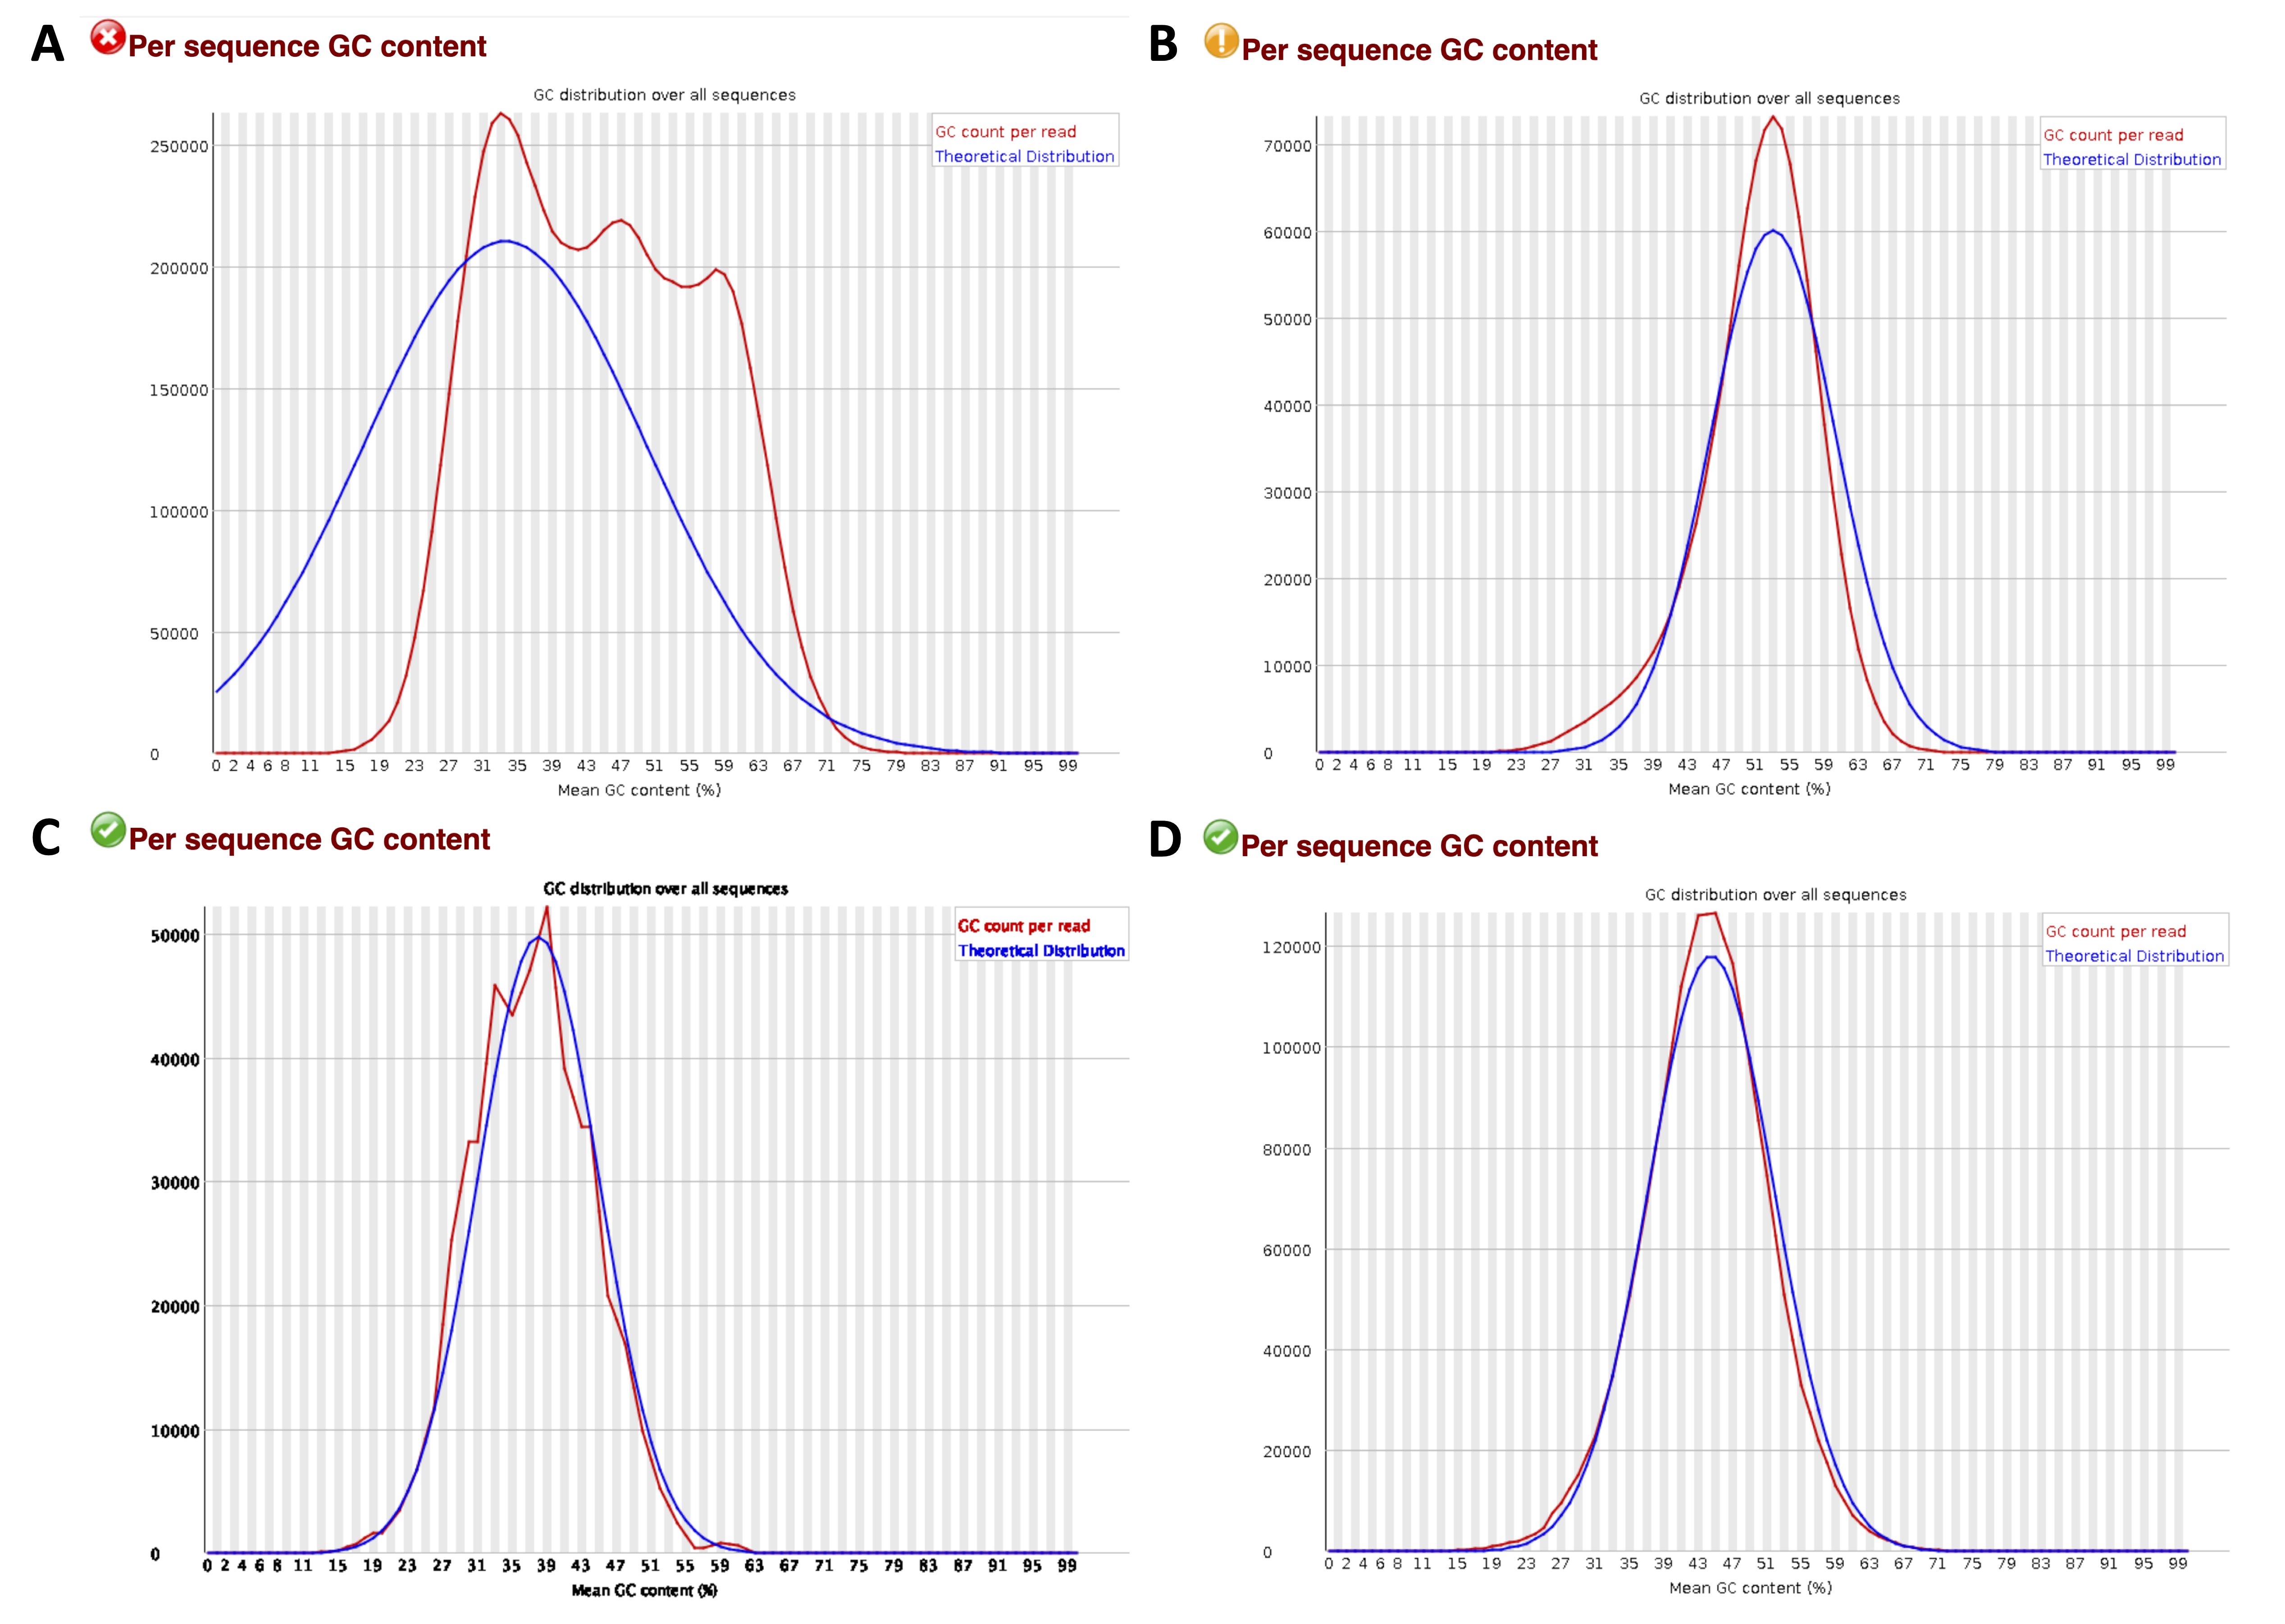
\includegraphics[scale=0.6]{fastqc}
    \caption{FastQC provides quality control measurements and visualizations for raw sequencing data, and is a near-universal first step in sequencing data analysis because of the insights it provides.
FastQC measures and summarizes 10 quality metrics and provides recommendations for whether the sample is within an acceptable quality range. In this figure, we show the per sequence GC content quality metric for \textbf{A} a metagenome with bacteria and archaea species. \textbf{B} \textit{Escherichia coli} isolate genome sequencing, \textbf{C} RAD-sequencing and \textbf{D} RNA-sequencing from \textit{Saccharomyces cerevisiae}. While the GC distribution shown in \textbf{A} would be concerning if the sample were from an isolate, it is acceptable and expected to see non-normal distributions for metagenomes.} 
    \label{fig:fastqc}
\end{figure}


%FastQC provides quality control measurements and visualizations for raw sequencing data, and is a near-universal first step in sequencing data analysis because of the insights it provides.
%FastQC measures and summarizes 10 quality metrics and provides recommendations for whether the sample is within an acceptable quality range. 
%The FastQC report is rich with information, both for prescribed and off-label interpretations. 
%For example, FastQC reports sequence length distribution, where the length of each read is plotted in a histogram. 
%For raw Illumina sequences, we expect a sharp peak where all reads are the same length; when there is variation in the length of sequences, we can infer that the reads have been trimmed in some way. 
%Another example is per sequence GC content. FastQC reports the percent content of GC nucleotides in the sequencing reads. 
%For single-species sequencing runs, we expect a smooth curve and a single peak. 
%If we observe multiple peaks, this may indicate that multiple species were sequenced in the sequencing run or that other abnormalities occurred during sequencing. 
%Many high-quality sequencing runs will fail FastQC metrics. 
%For example, we expect duplication levels to be high for RNA-sequencing or amplicon data. 
%Likewise, we expect multiple peaks in GC content for metagenomic data. 
%Insights gained using FastQC may not be definitive, but given the speed and computational tractability of the program, it is a rapid first-pass analysis to better understand the quality and content of the data that can be further tested by additional tools.}

\subsubsection*{Handling common biases in sequencing data} % this title isn't right yet, just trying to concisely summarize the all caps

There are many known biases in sequencing data. 
These biases originate from experimental design, methodology, sequencing chemistry, or workflows, and are helpful to target specifically with quality control measures. 
For example, PCR duplicates can cause problems in libraries that underwent an amplification step, and often need to be removed prior to downstream analysis. 
Nucleotide extraction kits have their own microbiomes (CITATION), so it may be important to check for specific contaminant sequences. 
Libraries sequenced with high concentrations of free adapters or with low concentration samples may have increased barcode hopping, leading to contamination between samples (CITATION). 
Stringent trimming of RNA-sequencing data may reduce isoform discovery (CITE MCMANNES). 
The exact biases in a specific data set or workflow will vary greatly between experiments. 
To determine what issues are most likely to plague your specific data set, it can be helpful to find recent publications using a similar experimental design, or to speak with experts at a sequencing core.


% this section is: some common issues to look for while doing QC. maybe _not_ greybox? bc most greyboxes are specific tools?
%\begin{greybox}{\subsection*{Finding and eliminating contaminant sequences} % 
\subsubsection*{Handling common contaminant sequences}
% maybe merge this section with the one above? (if can find right header)
Contamination in sequencing data can come from many sources. 
Many contaminants leave a detectable signal in sequencing data, allowing them to be removed, or in the worst cases, for libraries to be regenerated and resequenced. 
Below we discuss strategies for identifying and removing common sources of contamination.

\textbf{Checking adapter and barcode sequences}
All sequencing libraries have helper sequences like adapters and barcodes that allow the sequencer to keep track of and capture biological nucleotides. 
Typically, each sequencing library is sequenced with a single specific chemistry, meaning adapters and barcodes leave consistent traces within a sample. 
Sometimes, contaminant sequences will have different barcodes or adapters than the rest of the sequences, and these can be detected both by looking at the sequences and bioinformatically using a tool like BBMap or FastQC (among many others). 

\textbf{Removing PhiX}
PhiX is a common contaminant in Illumina sequencing data. Its used as a quality control spike-in in some sequencing runs. 
Many sequencing facilities remove PhiX before distributing sequencing data to their customers, but PhiX can still lurk in publicly available data or be inadvertently retained in new sequencing data. 
When working with new sequencing data, it’s a good idea to check for the presence of PhiX. 
This can be done using a tool like BLAST, aligning reads to the PhiX genome, or using k-mer baiting to pull reads that have k-mers in common with PhiX. 

\textbf{Removing human and host sequence}
Human DNA is a common contaminant given its ubiquity. 
Likewise, for microbiome experiments, DNA originating from the host organism can comprise a large portion of sequencing reads.
In both cases, it is often helpful to understand the proportion of reads attributable to human or host DNA. 
Both mapping and k-mer baiting are effective at removing these contaminants when a reference genome is available. 
When no reference genome is available, tetranucleotide frequency clustering and domain-specific marker gene annotation can help identify contaminant sequences (CITE or give ex).

\textbf{Ensuring correct species presence }
Often times, we have preconceived ideas of what species should be in our sequencing samples. 
For example, when sequencing a single genome, we expect only one species to be present. 
We recommend two general approaches for contaminant discovery: database looks up and marker-gene identification. 
Tools like sourmash, kraken, centrifuge, and MEGAN can be used to estimate the proportion of reads that match sequences in existing databases. 
Complementarily, marker-gene approaches like GraftM can quickly estimate the taxonomic composition of a sample based on single marker genes like 16s or 18s rRNA. 
These approaches can be applied to assembled sequences or reads. 
When no reference is available, tetranucleotide clustering of scaffolds or contiguous sequences can highlight contaminants (CITATION).%}
%\end{greybox}

Because sequencing data and applications are so diverse, there is no one-size-fits-all solution for quality control. 
Therefore, it is important to think critically about your expectations, and what patterns you expect to see given your data and your biological problem. 

\subsection*{Make big data less big} % heh. working title 

\subsubsection*{Build your workflow using subsampled data}
%You can begin this before generating your own data (if you're sequencing) by using similar publicly-available data to test a potential workflow. Once you have your data (public or freshly generated), the best test data can be directly created from your full dataset.

It is rare to find a workflow that will analyze your data from start to finish without testing, troubleshooting, and iteration.
To facilitate workflow design and save resources, you'll want to test each step with a small dataset prior to running your full analysis. 
After installing a program, if the program comes with test data, run it and check results against the expected results, to verify that it is working on your system. 
After that, subsample your own data and check you can run the program on this subsampled data. 
For example, if working with FASTQ data, you can subsample the first million lines of your data (first 250k reads) by running:

 \begin{lstlisting}
 head -n 1000000 FASTQ_FILE.fq > test_fastq.fq 
\end{lstlisting}

While there are many more sophisticated ways to subsample reads, this technique should be sufficient for testing each step of a workflow prior to running your full dataset. 
Note, some programs will fail with too few reads or too few results, so be sure to examine that possibility if running into errors at this stage, either in the literature, program manual, or by running larger subsets of data.
% add sentence here to reiterate concept of testing on public data!


\subsubsection*{Use computational approximations where possible}
 
 Many bioinformatics workflows take a long time and significant computational resources to run, and interpretable results are often only produced by the last few steps. 
This means that time-to-insight from sequencing data is often very high. 
 
%\subsubsection*{Generating quick insights with sketching algorithms}
%\textbf{Generating quick insights with sketching algorithms}

% one general paragraph re: approx, quantification,etc, one on sketching. maybe sketching first
Understanding the basic structure of data, the relationship between samples, and the approximate composition of each sample is very helpful at the beginning of data analysis, and can often drive analysis decisions in different directions than those originally intended. 
Although most bioinformatics workflows generate these types of insights, there are a few tools that do so rapidly, allowing the user to generate quick hypotheses that can be further tested by more extensive, fine-grained analyses. 

\textbf{Sketching} Sketching algorithms work with compressed approximate representations of sequencing data and thereby reduce runtimes and computational resources. 
These approximate representations retain enough information about the original sequence to recapitulate the main findings from many exact but computationally intensive workflows. 
Most sketching algorithms estimate sequence similarity in some way, allowing the user to gain insights from these comparisons.
For example, sketching algorithms can be used to estimate all-by-all sample similarity which can be visualized as a Principle Component Analysis or a multidimensional scaling plot, or can be used to build a phylogenetic tree with accurate topology. 
Sketching algorithms also dramatically reduce the runtime for comparisons against databases (e.g. all of GenBank), allowing users to quickly compare their data against large public databases. 
Sketching algorithms have been reviewed in-depth by Rowe \cite{rowe2019streaming}.

\textbf{Read Quantification vs Mapping}
%% had a thought - seems like we could briefly mentioning quantification vs read mapping here might be a good way to round out the "make big data less big" section
\textbf{Anything else to mention?}


\subsection*{Assess required resources}
% Use only the Resources you need / Calculating required resources
%\textbf{What resources do you actually need to use?} 

%It is difficult to assess the computational resources required to run different bioinformatic tools. 
Bioinformatic tools vary in the resources they require: some analysis steps are compute-intensive, other steps are memory intensive, and still others will have large intermediate storage needs. 
Tools will also vary in their ability to properly parallelize computation across multiple compute nodes. 
To minimize required computational resources for your analysis, it is worth assessing the resources required at each step.

Workflow software such as snakemake and nextflow provide avenues for specifying the resource needs of each individual step.

Some tools publish required resources for test and sample data either in a publication or in software manuals or readmes. 
However if this information is not available, its nearly impossible to estimate the amount of resources needed without running the tool. 
Monitoring resource usage (including RAM, CPUs, disk input and output, network usage, and time) while running the test data from a tool or on a subset of your data can give you a starting estimate for resource usage that you can scale up to accommodate the size of your actual data. 
Commands like "time" and "top" can help you monitor usage, while most workflow managers have built-in commands to report resource usage. 
Over time, you will develop a intuition for resource usage as you use more tools.


\section*{Troubleshooting: how to help yourself and when to get help}

If you have tried the strategies above and are having trouble with your data, it’s time to ask for help. 
The first point of attack is always to Google the error, including any identifying error message or code, the program name, and if necessary, the type of data you’re running. 
There are a vast array of online resources for bioinformatic help ranging from question sites such as Stack Overflow and BioStars, to personal or academic blogs or even tutorials and lessons written by experts in the field. 
In most cases, the error you’ve encountered has been encountered many times before, and often the solution is readily available. 
If you can’t find any solutions in the relevant search results, it’s time to escalate. 
If the error is with a specific program, it’s best to post on that program’s help or issue location (e.g. GitHub Issues), or google group mailing list. 
Often the authors of your software will post their preferred location for answering questions and solving errors related to their program. 
Be sure to include the relevant details of your error, including terminal output and the version of the software you are using.
 If your error or question is more general, such as asking about program choice or workflows, Stack Overflow is a good choice. 
First, search through related topics to ensure your question has not already been answered. 
If it hasn’t, make a post to a relevant section, and be sure to include all relevant information in your post - type of data you have, approaches you’ve tried already, relevant error message, etc. 

While there is lots of help available online, there’s no substitute for local communities where you can get help working with your data and learning to troubleshoot. 
Many people around you may be experiencing similar issues and finding it difficult to find appropriate help. 
Developing a local bioinformatics community, either via seminar series or meetup sessions for data analysis, can also help in both improving and expanding your work in this area. 
Once you establish a local community, it may also be useful to set up a local online sites (e.g. discourse) for group troubleshooting. 
While this may seem like just a local version of Stack Overflow, the local, member-only nature can help create a safe and collaborative online space for troubleshooting problems often encountered by your local bioinformatics community. 
The benefit to beginners is clear: learning the best way to post questions and the important parts of errors, while getting their questions answered so they can move forward in their research. 
However, intermediate users may find these communities most useful, as they can also accelerate their own troubleshooting skills by helping others solve issues that they have already struggled through. 
While it can be helpful to have some “experts” available to help answer questions or to know when to escalate to Stack Overflow or other communities, a collaborative community of practice with members at all experience levels can help all its members move their science forward faster.


% For figure citations, please use "Fig" instead of "Figure".

%Nulla mi mi, Fig~\ref{fig1} venenatis sed ipsum varius, volutpat euismod diam. Proin rutrum vel massa non gravida. Quisque tempor sem et dignissim rutrum. Lorem ipsum dolor sit amet, consectetur adipiscing elit. Morbi at justo vitae nulla elementum commodo eu id massa. In vitae diam ac augue semper tincidunt eu ut eros. Fusce fringilla erat porttitor lectus cursus, \nameref{S1_Video} vel sagittis arcu lobortis. Aliquam in enim semper, aliquam massa id, cursus neque. Praesent faucibus semper libero.

% Place figure captions after the first paragraph in which they are cited.
%\begin{figure}[!h]
%\caption{{\bf Bold the figure title.}
%Figure caption text here, please use this space for the figure panel descriptions instead of using subfigure commands. A: Lorem ipsum dolor sit amet. B: Consectetur adipiscing elit.}
%\label{fig1}
%\end{figure}

% Results and Discussion can be combined.
%\section*{Results}
%Nulla mi mi, venenatis sed ipsum varius, Table~\ref{table1} volutpat euismod diam. Proin rutrum vel massa non gravida. Quisque tempor sem et dignissim rutrum. Lorem ipsum dolor sit amet, consectetur adipiscing elit. Morbi at justo vitae nulla elementum commodo eu id massa. In vitae diam ac augue semper tincidunt eu ut eros. Fusce fringilla erat porttitor lectus cursus, vel sagittis arcu lobortis. Aliquam in enim semper, aliquam massa id, cursus neque. Praesent faucibus semper libero.


%PLOS does not support heading levels beyond the 3rd (no 4th level headings).
%\subsection*{\lorem\ and \ipsum\ nunc blandit a tortor}
%\subsubsection*{3rd level heading} 
%Maecenas convallis mauris sit amet sem ultrices gravida. Etiam eget sapien nibh. Sed ac ipsum eget enim egestas ullamcorper nec euismod ligula. Curabitur fringilla pulvinar lectus consectetur pellentesque. Quisque augue sem, tincidunt sit amet feugiat eget, ullamcorper sed velit. Sed non aliquet felis. Lorem ipsum dolor sit amet, consectetur adipiscing elit. Mauris commodo justo ac dui pretium imperdiet. Sed suscipit iaculis mi at feugiat. 

%\begin{enumerate}
%	\item{react}
%	\item{diffuse free particles}
%	\item{increment time by dt and go to 1}
%\end{enumerate}

%\begin{itemize}
%	\item First bulleted item.
%	\item Second bulleted item.
%	\item Third bulleted item.
%\end{itemize}

\section*{Conclusion}

%CO\textsubscript{2} 
% For more information, see \nameref{S1_Appendix}.

\section*{Supporting information}

% Include only the SI item label in the paragraph heading. Use the \nameref{label} command to cite SI items in the text.
%\paragraph*{S1 Fig.}
%\label{S1_Fig}
%{\bf Bold the title sentence.} Add descriptive text after the title of the item (optional).

%\paragraph*{S2 Fig.}
%\label{S2_Fig}
%{\bf Lorem ipsum.} Maecenas convallis mauris sit amet sem ultrices gravida. Etiam eget sapien nibh. Sed ac ipsum eget enim egestas ullamcorper nec euismod ligula. Curabitur fringilla pulvinar lectus consectetur pellentesque.

%\paragraph*{S1 File.}
%\label{S1_File}
%{\bf Lorem ipsum.}  Maecenas convallis mauris sit amet sem ultrices gravida. Etiam eget sapien nibh. Sed ac ipsum eget enim egestas ullamcorper nec euismod ligula. Curabitur fringilla pulvinar lectus consectetur pellentesque.

%\paragraph*{S1 Video.}
%\label{S1_Video}
%{\bf Lorem ipsum.}  Maecenas convallis mauris sit amet sem ultrices gravida. Etiam eget sapien nibh. Sed ac ipsum eget enim egestas ullamcorper nec euismod ligula. Curabitur fringilla pulvinar lectus consectetur pellentesque.

%\paragraph*{S1 Appendix.}
%\label{S1_Appendix}
%{\bf Lorem ipsum.} Maecenas convallis mauris sit amet sem ultrices gravida. Etiam eget sapien nibh. Sed ac ipsum eget enim egestas ullamcorper nec euismod ligula. Curabitur fringilla pulvinar lectus consectetur pellentesque.

%\paragraph*{S1 Table.}
%\label{S1_Table}
%{\bf Lorem ipsum.} Maecenas convallis mauris sit amet sem ultrices gravida. Etiam eget sapien nibh. Sed ac ipsum eget enim egestas ullamcorper nec euismod ligula. Curabitur fringilla pulvinar lectus consectetur pellentesque.

\section*{Acknowledgments}
thanks thanks thanks thanks

\nolinenumbers

% Either type in your references using
% \begin{thebibliography}{}
% \bibitem{}
% Text
% \end{thebibliography}
%
% or
%
% Compile your BiBTeX database using our plos2015.bst
% style file and paste the contents of your .bbl file
% here. See http://journals.plos.org/plosone/s/latex for 
% step-by-step instructions.
% 

% this compiles our bibliography.bib file and inserts references here
%not sure if we need to paste refs in prior to submission, see http://journals.plos.org/plosone/s/latex
\bibliography{bibliography}

\end{document}

